\chapter{Bessel functions}
\label{h:bessel}

\begin{quote}
\noindent\marginnote{Bessel obviously had many qualities, but unfortunately, leaving memorable quotes to posterity does not seem to have been one of them...}We must admit with humility that, while number is purely a product of our minds, space has a reality outside our minds, so that we cannot completely prescribe its properties a priori.

-- Carl Friedrich Gauss, letter to Bessel
\end{quote}

\chaptertoc

In this chapter, we will look at Bessel functions and their cousins the Neumann and the Hankel functions. These naturally occur when solving problems in cylindrical coordinate systems. 

After presenting their corresponding differential equation, we introduce a different way of defining these functions based on so-called generating functions. These are useful to more easily prove all sorts of useful properties, like recurrence relationships. Additionally, we will tackle integrals involving Bessel functions, as well as use them in series expansions. Finally, we apply our newfound knowledge to the problem of finding modes in an optical fibre.


\pagebreak


\sectionugent{Bessel's differential equation}\label{sec-bessel-eq}

\begin{marginfigure}[.3cm]
  % credits: Wikipedia
  % url: https://en.wikipedia.org/wiki/Daniel_Bernoulli 
  \includegraphics{bessel/figures/d_bernouilli}
  \caption{Daniel Bernouilli (1700-1782)}
\end{marginfigure}

Let's take a look at the scalar Helmholtz equation, which describes wave propagation in a medium with constant refractive index $n$, where the wavevector in vacuum is given by $k_0=2 \pi / \lambda_0$:

\begin{equation}
\nabla^2 \psi  + k_0^2 n^2 \psi = 0 
\end{equation}

Converting this to cylindrical coordinates gives us

\begin{equation}
\frac{\partial^2 \psi}{\partial r^2} + \frac{1}{r} \frac{\partial \psi}{\partial r} +\frac{1}{r^2} \frac{\partial^2 \psi}{\partial \theta^2} + \frac{\partial^2 \psi}{\partial z^2} + k_0^2 n^2\psi = 0 \label{eq-helmholtz-cyl}
\end{equation}

Let's try a solution of the following form, with $k_\theta$ and $k_z$ constant: 

\begin{equation}
\psi(r,\theta,z) = R(r)e^{-j k_\theta \theta }e^{-j k_z z}
\label{eq-bessel-ansatz}
\end{equation}  

(Later in this chapter, we will look at the physical interpretation behind this expression. For now, just assume that the form of this trial solution is a flash of divine inspiration.)

\begin{cue}
Substitute Eq.~\ref{eq-bessel-ansatz} in Eq.~\ref{eq-helmholtz-cyl}.
\end{cue}

This leads to

\begin{equation}
\frac{d^2 R(r)}{d r^2} + \frac{1}{r} \frac{d R(r)}{d r} + \left[k_0^2 n^2 - k_z^2 - \frac{k_\theta^2}{r^2} \right] R(r) = 0
\end{equation} 


\begin{equation}
r^2\frac{d^2 R(r)}{d r^2} + r \frac{d R(r)}{d r} + \left[ r^2 (k_0^2 n^2 - k_z^2)- k_\theta^2 \right] R(r) = 0
\end{equation}

Let's make this a little bit more generic, without explicit references to the Helmholtz equation.

For that, we can rename $R$ to $X$ and $k_\theta$ to $\nu$, as well as make the following change of variables

\begin{equation}
x = r \sqrt{k_0^2 n^2 - k_z^2} \stackrel{def}{=} k_t r
\end{equation}

\begin{cue}
Implement those changes.
\end{cue}

We know that

\begin{equation}
 \frac{d}{d r} =  \frac{d}{d x} \frac{dx}{dr} = k_t \frac{d}{d x} 
\end{equation}

After some algebraic manipulation, this leads to

\begin{equation}
\fbox{$\displaystyle
x^2\frac{d^2 X(x)}{d x^2} + x \frac{d X(x)}{d x} + \left(x ^ 2 - \nu^2 \right)X(x) = 0 \label{eq-bessel}
$}
\end{equation}

\noindent\marginnote{D. Bernoulli was the first one to work with what we now call $J_0(x)$. Bessel later generalised this to other orders.}Eq.~\ref{eq-bessel} is called Bessel's differential equation. A solution to this equation is given by $J_\nu(x)$, the Bessel function of the first kind of order $\nu$.

In what follows, we will mostly consider the important special case where $\nu$ is an integer. In this situation, we will use the notation $J_n(x)$, where $n$ is the integer version of $\nu$ and is not to be confused with the refractive index $n$ in Eq.~\ref{eq-helmholtz-cyl}.


\pagebreak


\sectionugent{Generating function for Bessel functions}

One way of figuring out what these Bessel functions look like, would be to propose a Taylor series expansion, substitute that into the differential equation, and then derive the expansion coefficients.

However, here we'll shift gears and take a completely different approach to define Bessel functions (at least for integer order). This will put an extra tool in our box that will help us derive some useful identities. Later on, we'll show that this new approach is equivalent to the original differential equation.

\noindent\marginnote{This is a purely mathematical trick. $t$ does not represent time, and in fact has no physical meaning at all.}Let's introduce a function of two variables, a so-called \emph{generating function}:

\begin{equation}
g(x,t) \stackrel{def}{=} e^{x/2(t-1/t)} \label{eq-gen-bessel}
\end{equation}

When we expand this function in a Laurent series in $t$, we \emph{define} the coefficients as being the Bessel functions:

\begin{equation}
\fbox{$\displaystyle
 g(x,t) =   e^{x/2(t-1/t)}  \stackrel{def}{=} \sum_{n = - \infty}^{\infty} J_n(x)t^n
    $}
  \label{eq-g-bessel}
\end{equation}

\begin{marginfigure}[-2cm]
  % credits: Wikimedia
  % url: https://commons.wikimedia.org/wiki/File:Friedrich_Wilhelm_Bessel_-_EESachse.jpg
  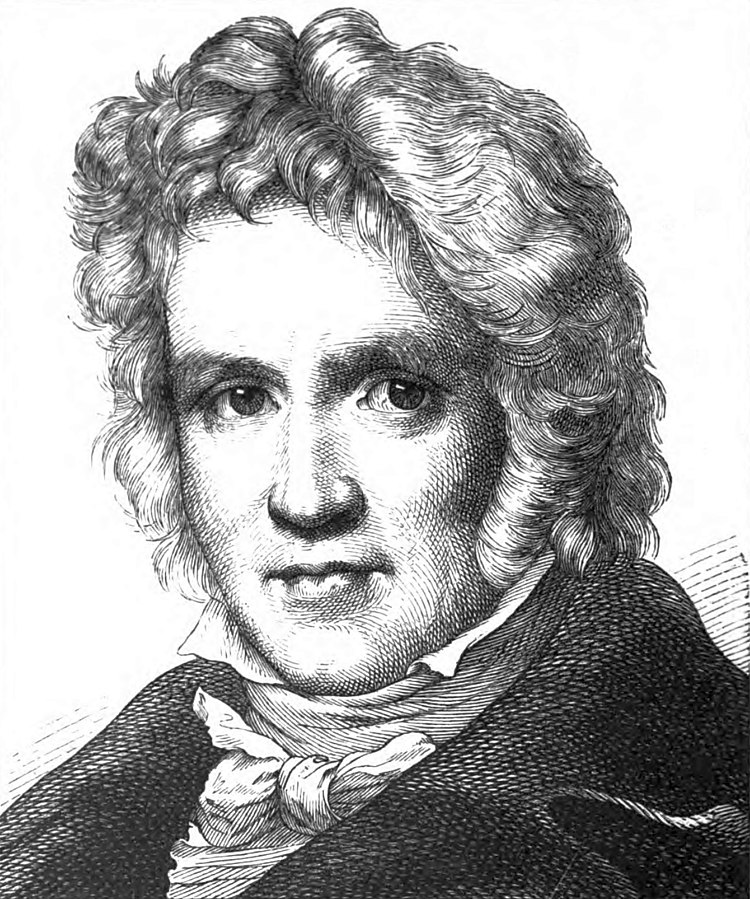
\includegraphics{bessel/figures/f_bessel}
  \caption{Friedrich Wilhelm Bessel (1784-1846)}
\end{marginfigure}

\begin{cue}
By expanding the exponentials in the equation above, derive a series expansion for $J_n(x)$.  
\end{cue}

Expanding the exponentials in Eq.~\ref{eq-g-bessel} gives us

\begin{equation}
e^{xt/2} \cdot e^{-x/2t} = \sum_{r = 0}^{\infty} {\left(\frac{x}{2}\right)}^r \frac{t^r}{r!} \cdot \sum_{s = 0}^{\infty} {(-1)}^s { \left(\frac{x}{2}\right)}^s \frac{t^{-s}}{s!}
\end{equation} 

Note that it is important to have a separate summation index for the series expansion of each of the two exponentials in the product. These are completely independent, and should be treated at such.

\noindent\marginnote{There is some subtlety in the lower bound of $s$, which is clear from e.g. the graphical interpretation of the product of the two series. See the video for more details.}Introducing a new variable $n = r - s$ and getting rid of $r$, we can reorganise this equation to give

\begin{equation}
e^{xt/2} \cdot e^{-x/2t} = \sum_{n = -\infty}^{\infty} \left[ \sum_{s = 0}^{\infty} {\left(\frac{x}{2}\right)}^{n+s} \frac{1}{(n+s)!} \cdot (-1)^s {\left(\frac{x}{2}\right)}^{s} \frac{1}{s!} \right] t^n
\end{equation} 

This means that

\begin{equation}
J_n(x) = \sum_{s = 0}^{\infty} \frac {{(-1)}^s}{s!(n+s)!} {\left(\frac{x}{2}\right)}^{n+2s} \label{eq-bessel-series}
\end{equation} 

This series expansion can be used to numerically calculate the Bessel functions. Fig.~\ref{fig-bessel-J} plots $J_0(x)$, $J_1(x)$, $J_2(x)$. As you can see, these functions oscillate, but are not periodic. Apart from $J_0$, all other orders are zero at the origin.

\begin{figure}
\centering
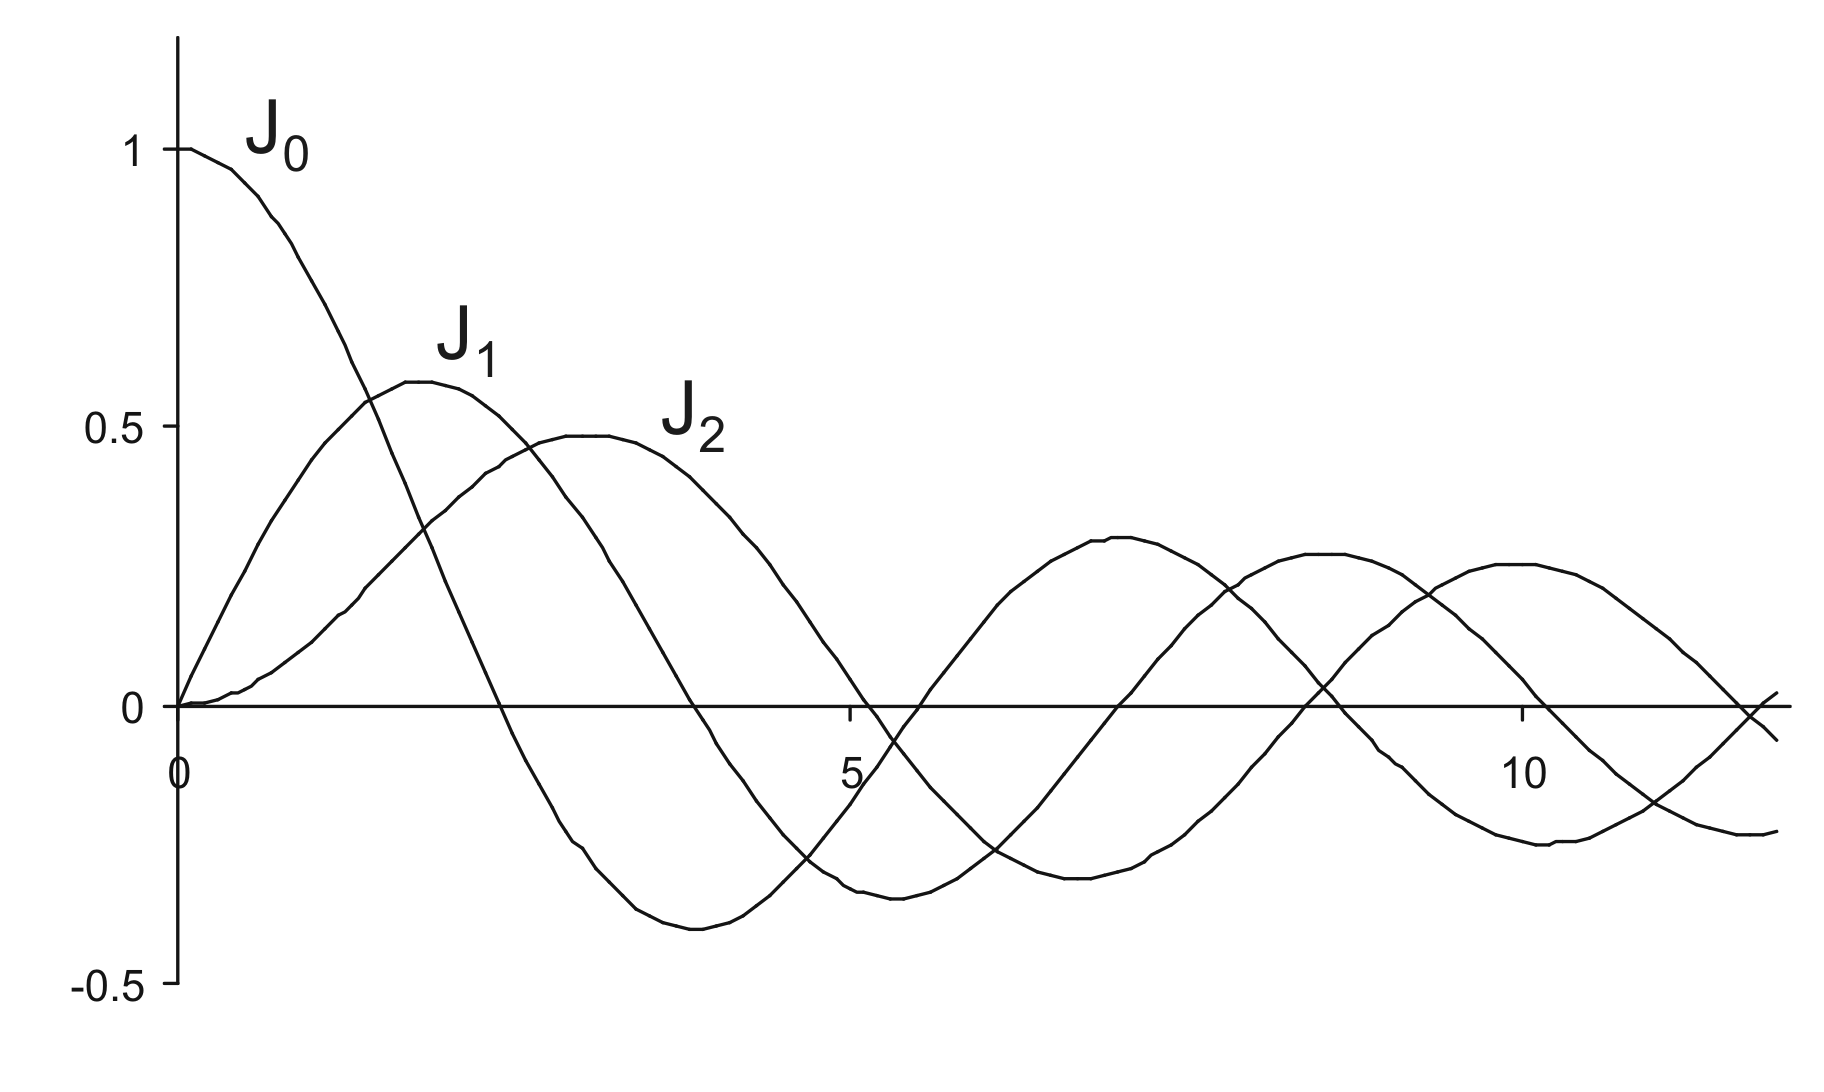
\includegraphics{bessel/figures/j}
\caption{The Bessel functions $J_0(x)$, $J_1(x)$ and $J_2(x)$.}
\label{fig-bessel-J}
\end{figure}

\begin{exer}
% difficulty: normal
Use the series expansion of Bessel functions to show that
$$\lim_{x \to 0} \frac{J_1(x)}{x}= \frac{1}{2}$$
\end{exer}

\begin{exer}
% difficulty: trivial
% ugent
By replacing $t$ by $-1/t$ in the generating function Eq.~\ref{eq-g-bessel}, show that
$$J_{-n}(x)=(-1)^nJ _n(x)$$
\end{exer}

\begin{exer}
% difficulty: normal
Use the product of the generating functions $g(x,t)$ and $g(x,-t)$ to show that
$$\left[ J_0(x) \right]^2 + 2 \sum_{n=1}^\infty \left[ J_n(x) \right]^2 = 1 $$
\end{exer}

\pagebreak

\begin{exer}
% difficulty: normal
Evaluate the following contour integral along the unit circle in the complex $t$-plane:

$$ \oint_C t^{-n-1} g(x,t) dt $$

In doing so, derive the following equations:

$$J_n(x) = \frac {1}{2\pi} \int_0 ^ {2 \pi} \cos (n \theta - x \sin \theta ) d\theta $$

$$ J_0(x) =  \frac {1}{2\pi} \int_0 ^ {2 \pi}  e^{j x \cos \theta} d \theta $$
\end{exer}

\begin{exer}
% difficulty: hard
By evaluating the generation function in a suitable point, prove the following
$$ \cos x =  J_0(x) + 2 \sum_{n=1}^\infty (-1)^n J_{2n}(x)  $$
$$ \sin x =  2 \sum_{n=0}^\infty (-1)^n J_{2n+1}(x)  $$
\begin{hnt}
Put $t=j$, take the real and imaginary parts.
\end{hnt}
\end{exer}


\pagebreak


\sectionugent{Recurrence relations for Bessel functions}

\begin{cue}
Differentiate the generating function with respect to $t$, and then resubstitute the generating function into the resulting expression. 
\end{cue}

If we differentiate Eq.~\ref{eq-g-bessel} with respect to $t$, we get

\begin{equation}
\frac{x}{2}\left({1 + \frac{1}{t^2}}\right) e^{x/2(t-1/t)} = \sum_{n = - \infty}^{\infty} n J_n(x)t^{n-1}
\end{equation}

Substituting Eq.~\ref{eq-g-bessel} back into this, we get

\begin{equation}
\frac{x}{2}\left({1 + \frac{1}{t^2}}\right) \sum_{n = - \infty}^{\infty} J_n(x)t^n = \sum_{n = - \infty}^{\infty} n J_n(x)t^{n-1}
\end{equation}

\begin{cue}
Use this to derive a relationship between $J_{n-1}(x)$, $J_{n-1}(x)$ and  $J_{n+1}(x)$. 
\end{cue}

\noindent\marginnote{If you'd like more intermediate steps here, have a look at the video.}Equating the coefficients of like powers of $t$, we get

\begin{equation}
\frac{x}{2} J_n(x) + \frac{x}{2} J_{n+2}(x) = (n+1)J_{n+1}(x)
\end{equation} 

Or with the substitution $n+1 \to n$

\begin{equation}
J_{n-1}(x) + J_{n+1}(x) = \frac{2n}{x} J_n(x)
\end{equation} 

\begin{exer}
% difficulty: trivial
% ugent
Differentiate the generating function with respect to $x$ to show that
$$ J_{n-1}(x) - J_{n+1}(x) = 2 J_n'(x)$$ \label{ex-recur}
\end{exer}


\begin{exer}
% difficulty: trivial
% ugent
Show that
$$\begin{array}{lcll}a) & J_{n-1}(x) = \frac{n}{x}J_n(x) + J_n'(x) \\b) & J_{n+1}(x) = \frac{n}{x}J_n(x) - J_n'(x) \\c) & \frac{d}{dx}\left[x^n J_n(x)\right] = x^n J_{n-1}(x) \\d) & \frac{d}{dx}\left[x^{-n} J_n(x)\right] = -x^{-n} J_{n+1}(x)\end{array}$$ \label{ex-recurrence}
\end{exer}

\pagebreak

\begin{exer}
% difficulty: normal
First, show that
$$\int_0^\infty J_1( x) dx =  1$$
Then, extend this to show that
$$\int_0^\infty J_1( x) dx = \int_0^\infty J_3( x) dx = \int_0^\infty J_5( x) dx = \cdots = 1$$
\end{exer}

\begin{exer}
% difficulty: normal
% ugent
Show that
$$\int_0^1 x^3 J_0(k x) dx =  \frac{J_1(k)}{k} - 2 \frac{J_2(k)}{k^2}$$
If $k$ is a zero of $J_0$, show that this integral is equal to
$$\frac{J_1(k)}{k^3}\left(k^2-4\right)$$
\end{exer}

\begin{exer}
% difficulty: hard
Fraunhofer diffraction is governed by the following equation:

$$U(x_0, y_0) \sim \iint_{-\infty}^{\infty} U(x_1, y_1) e ^{j \frac{2\pi}{\lambda z} (x_0 x_1 + y_0 y_1)} dx_1 dy_1  $$

By using polar coordinates both in the aperture plane

$$x_1 = \rho_1 \cos \theta_1; \quad y_1 = \rho_1 \sin \theta_1$$

and the observation plane

$$x_0 = \rho_0 \cos \theta_0; \quad y_0 = \rho_0 \sin \theta_0$$

show that for rotationally symmetric apertures this reduces to

$$U(\rho_0) \sim  \int_0^{\infty} \int_0^{2 \pi} U(\rho_1)  e ^{j \frac{2\pi}{\lambda z} \rho_0 \rho_1 \cos \theta_1} \rho_1 d\rho_1 d\theta_1  $$

\begin{marginfigure}[-5cm]
  % credits: Wikipedia
  % url: https://en.wikipedia.org/wiki/George_Biddell_Airy 
  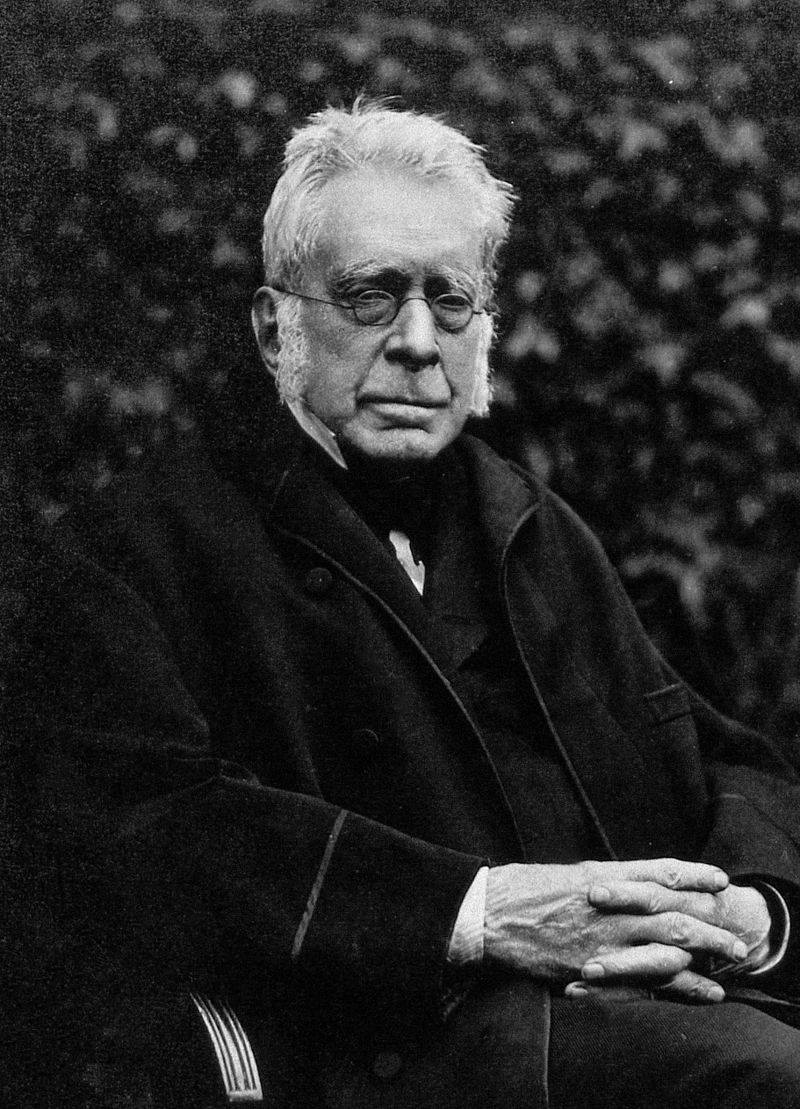
\includegraphics{bessel/figures/g_airy}
  \caption{George Biddell Airy (1801 – 1892)}
\end{marginfigure}

Then, proceed to calculate the so-called Airy diffraction pattern for a circular aperture of radius $a$:

$$U(\rho_0) \sim \frac {J_1\left( 2 \pi \frac {\rho_0 a}{\lambda z} \right)}{\frac{\rho_0}{\lambda z a}}$$

\end{exer}


\section{Bessel's differential equation revisited}

The aim of this section is to show that a function defined using the generating function for Bessel functions, satisfies Bessel's differential equation. We will achieve this by doing some mathematical gymnastics, starting from the recurrence relationships we derived using the generating function.

Let's begin with one of the results from Exer. \ref{ex-recurrence}:

\begin{equation}
J_{n-1}(x) = \frac{n}{x}J_n(x) + J_n'(x)
\end{equation}

\begin{cue}
Multiply this by $x$, take the derivative with respect to $x$, and multiply by $x$ again.
\end{cue}

Getting rid of the denominator, this can be written as

\begin{equation}
x J_n'(x) + n J_n(x) - x J_{n-1}(x) = 0 \label{eq-bessel-dif-rec}
\end{equation} 

Differentiating with respect to $x$, we get

\begin{equation}
J_n'(x) + x J_n''(x) + n J_n'(x) - J_{n-1}(x) - x J_{n-1}'(x)= 0
\end{equation} 

or, after multiplying by $x$:

\begin{equation}
x^2 J_n''(x) + (n + 1) x J_n'(x) - x J_{n-1}(x) - x^2 J_{n-1}'(x)= 0
\end{equation} 

\begin{cue}
From this equation, subtract Eq.~\ref{eq-bessel-dif-rec} multiplied by $n$.
\end{cue}

Subtracting Eq.~\ref{eq-bessel-dif-rec} multiplied by $n$:

\begin{align}
x^2 J_n''(x) +& (n + 1) x J_n'(x) - x J_{n-1}(x) - x^2 J_{n-1}'(x) \nonumber \\-& n\left(x J_n'(x) + n J_n(x) - x J_{n-1}(x)\right)= 0
\end{align} 

This simplifies to

\begin{equation}
x^2 J_n''(x) +  x J_n'(x) - x^2 J_{n-1}'(x) - n^2 J_n(x) + (n - 1) x J_{n-1}(x)= 0 \label{eq-bessel-dif-rec-2}
\end{equation} 

As a next step, we now take another recurrence equation from Exer. \ref{ex-recurrence}:

\begin{equation}
J_{n+1}(x) = \frac{n}{x}J_n(x) - J_n'(x)
\end{equation} 

\begin{cue}
In the equation above, replace $n$ with $n-1$, and use the result to eliminate $J_{n-1}$ and $J_{n-1}'$ from Eq.~\ref{eq-bessel-dif-rec-2}.
\end{cue}

Replacing $n$ with $n-1$, this can be written as

\begin{equation}
x J_{n}(x) = (n-1)J_{n-1}(x) - x J_{n-1}'(x)
\end{equation} 

With this, we can eliminate $J_{n-1}$ and $J_{n-1}'$ from Eq.~\ref{eq-bessel-dif-rec-2}:

\begin{equation}
x^2 J_n''(x) +  x J_n'(x) + x^2 J_n(x) - n^2 J_n(x) = 0
\end{equation} 

This is nothing other than Bessel's differential equation Eq.~\ref{eq-bessel}.

This shows that any function satisfying the recurrence relations used, also satisfies Bessel's equation.


\pagebreak


\sectionugent{Lommel's integral}

Bessel functions can be used as a basis set for a series expansion of an arbitrary function. Before we can tackle this, we require some orthogonality relations for which we need to calculate a certain type of integral.

\begin{marginfigure}[-.0cm]
  % credits: Wikipedia
  % url: https://en.wikipedia.org/wiki/Eugen_von_Lommel
  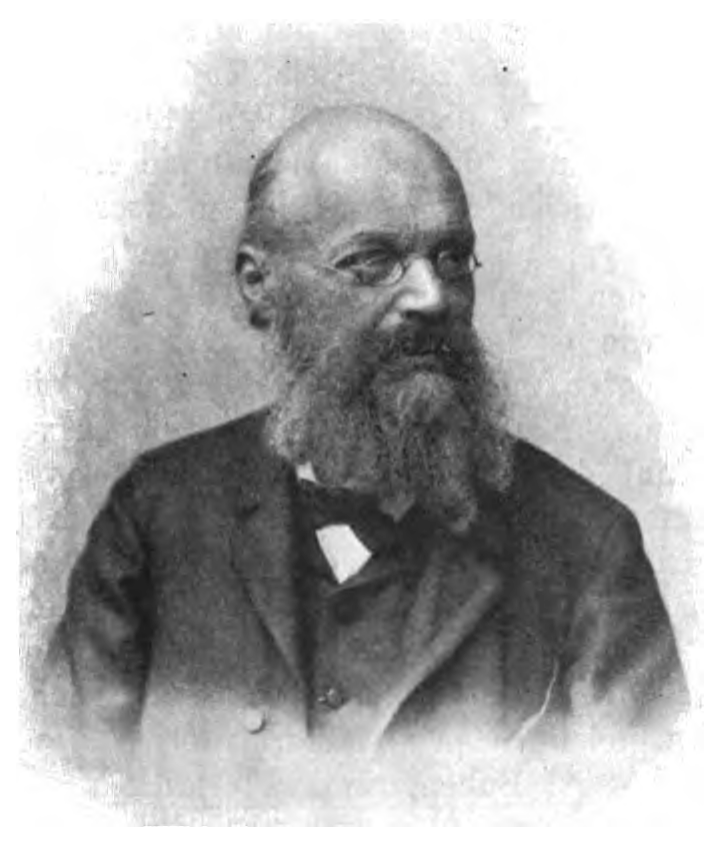
\includegraphics{bessel/figures/e_lommel}
  \caption{Eugen von Lommel (1837-1899)}
\end{marginfigure}

Consider the following two differential equations:

\begin{equation}
x^2 \frac{d^2 \phi}{dx^2}  + x \frac{d \phi}{dx} + \left(l^2x^2 - n^2\right) \phi = 0 \label{eq-bessel-orth-1}
\end{equation} 

\begin{equation}
x^2 \frac{d^2 \psi}{dx^2}  + x \frac{d \psi}{dx} + \left(k^2x^2 - n^2\right) \psi = 0 \label{eq-bessel-orth-2}
\end{equation}

\begin{cue}
What are the solutions to these equations?  
\end{cue}

Solutions to these equations are $J_n(lx)$ and $J_n(kx)$ respectively.

\begin{cue}
Multiplying Eq.~\ref{eq-bessel-orth-1} with $\psi/x$, Eq.~\ref{eq-bessel-orth-2} with $\phi/x$ and subtract the two results.  
\end{cue}

By multiplying Eq.~\ref{eq-bessel-orth-1} with $\psi/x$, Eq.~\ref{eq-bessel-orth-2} with $\phi/x$ and subtracting the two results, we get

\begin{equation}
x \left( \frac{d^2 \phi}{dx^2}\psi - \frac{d^2 \psi}{dx^2} \phi \right) + \left(\psi \frac{d \phi}{dx}- \frac{d \psi}{dx}\phi\right) + \left(l^2 - k^2\right) x \phi \psi = 0
\end{equation}

\begin{cue}
Look at the first two terms of the equation above, and try to write them as a total differential. 
\end{cue}

This can be written as

\begin{equation}
\frac{d}{dx}\left[x \left( \frac{d \phi}{dx} \psi - \frac{d \psi}{dx} \phi\right)\right] = \left(k^2 - l^2\right) x \phi \psi
\end{equation}

such that

\begin{align}
x \left[{\frac{dJ_n(lx)}{dx}  J_n(kx) - \frac{dJ_n(kx)}{dx} J_n(lx)}\right] + C = \nonumber \\ \left(k^2 - l^2\right)\int x J_n(lx)J_n(kx)dx
\end{align}

\begin{cue}
To clean this up, write this in terms of $J_n'(kx)$ and  $J_n'(lx)$, where the prime symbol denotes derivation with respect to the \emph{entire} argument. 
\end{cue}

We have $dJ_n(kx)/dx = kJ_n'(kx)$ and $dJ_n(lx)/dx = lJ_n'(lx)$, such that for $l \ne \pm k$

\begin{align}
  \int x & J_n(lx)J_n(kx)dx = \nonumber \\
  & \frac{x}{k^2 - l^2} \left[{l J_n'(lx) J_n(kx) -  k J_n'(kx) J_n(lx)}\right] + C \label{eq-lommel-1}
\end{algin} 

\begin{cue}
Use one of the recurrence relationships to get rid of the derivative, paying the price of introducing terms with Bessel functions of order $n+1$.
\end{cue}

The second recurrence relation from Exer. \ref{ex-recurrence} takes the form

\begin{equation}
J_n'(lx) =  \frac{n}{lx}J_n(lx)-J_{n+1}(lx)
\end{equation} 

Likewise,
\begin{equation}
J_n'(kx) =  \frac{n}{kx}J_n(kx)-J_{n+1}(kx)
\end{equation} 

So, Eq.~\ref{eq-lommel-1} becomes

\begin{align}
  \int x & J_n(lx)J_n(kx)dx = \nonumber \\
  & \frac{x}{k^2 - l^2} \left[{k J_{n+1}(kx) J_n(lx) - l J_{n+1}(lx) J_n(kx)}\right] + C \label{eq-lommel-2}
\end{align} 

Eq.~\ref{eq-lommel-2} is called Lommel's integral.


\pagebreak


\sectionugent{Fourier--Bessel series}

Let's now play around with Lommel's integral.

\begin{marginfigure}[-.3cm]
  % credits: Wikipedia
  % url: https://en.wikipedia.org/wiki/Joseph_Fourier
  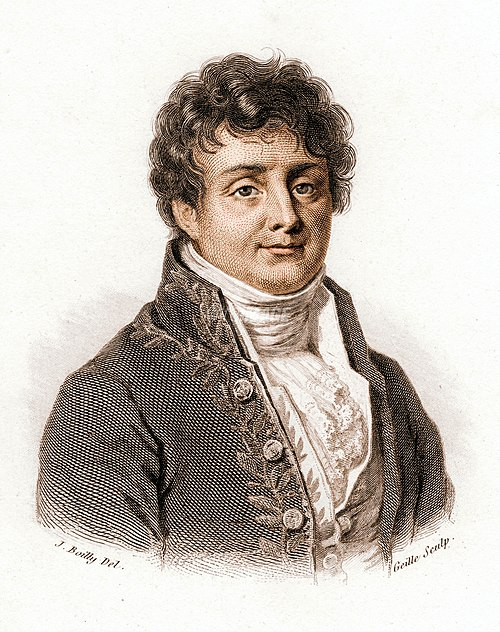
\includegraphics{bessel/figures/j_fourier}
  \caption{Jean-Baptiste Joseph Fourier (1768–1830)}
\end{marginfigure}

Suppose that $\xi_i$ and $\xi_j$ are two different zeros of $J_n(x)$. Then, from Lommel's integral Eq.~\ref{eq-lommel-2}, it immediately follows that

\begin{equation}
\fbox{$\displaystyle
\int_0^1 x J_n(\xi_i x)J_n(\xi_j x)dx = 0 \label{eq-bessel-ortho}
$}
\end{equation} 

This can be seen as an orthogonality condition that $J_n(\xi_i x)$ and $J_n(\xi_j x)$ satisfy, at least when we define a scalar product in a creative way, using a weighting function $x$:

\begin{equation}
\left<f(x),g(x)\right> \stackrel{def}{=} \int_0^1 x f(x) g(x) dx
\end{equation} 

\noindent\marginnote{One can prove that all zeros $\xi_i$ are real and that there is an infinite number of them.} Eq.~\ref{eq-bessel-ortho} can be used to expand functions in a so--called \emph{Fourier--Bessel} series. Suppose $\xi_i$ is the set of zeros of $J_n(x)$. For a function $f(x)$ defined in the interval $[0,1]$, we can write:

\begin{equation}
f(x) = \sum_{i=0}^{\infty} a_i J_n(\xi_i x) \label{eq-fourier-bessel}
\end{equation} 

To determine the unknown coefficients $a_i$, we multiply Eq.~\ref{eq-fourier-bessel} by $x J_n(\xi_m x)$ and integrate over $[0,1]$.

\begin{cue}
Perform these operations and make use of the orthogonality relation to determine the expansion coefficients.  
\end{cue}

Thanks to the orthogonality relations, we get

\begin{equation}
\int_0^1 x J_n(\xi_m x) f(x) dx = a_m \int_0^1 x J_n^2(\xi_m x) dx \label{eq-fourier-bessel-2}
\end{equation} 

The integral on the left--hand side of Eq.~\ref{eq-fourier-bessel-2} can be calculated analytically or numerically, depending on the nature of $f(x)$. To evaluate the integral on the right--hand side of \ref{eq-fourier-bessel-2}, we cannot use Lommel's integral Eq.~\ref{eq-lommel-2}, because $k=l$. So we need to calculate this normalisation integral in a different way, which we will do now.

We need to calculate

\begin{equation}
I = \int x J_n^2(k x) dx
\end{equation}

\begin{cue}
Make the change of variables $kx = t$ and perform integration by parts.
\end{cue}

After a change of variables $kx = t$, this becomes

\begin{equation}
I = \frac{1}{k^2} \int t J_n^2(t) dt
\end{equation}

Integration by parts, with $u=J_n^2(t)$ and $dv=t dt$, yields

\begin{equation}
I = \frac{t^2}{2 k^2}J_n^2(t) - \frac{1}{k^2} \int t^2 J_n(t) J_n'(t) dt
\end{equation}

\begin{cue}
  To solve the remaining integral, write down that $J_n(t)$ satisfies Bessel's differential equation. Multiply the result by $J_n'(t)$, and use this to write $t^2 J_n(t) J_n'(t)$ as a total differential. 
\end{cue}

Because $J_n(t)$ is a solution of Bessel's equation Eq.~\ref{eq-bessel}, we can write

\begin{equation} 
- t^2 J_n(t) = t^2 J_n''(t) + t J_n'(t) - n^2 J_n(t)
\end{equation}

Multiplying this by $J_n'(t)$ we get

\begin{align} 
- t^2 J_n(t) J_n'(t) = &\, t^2 J_n''(t)J_n'(t) + t J_n'^2(t) - n^2 J_n(t)J_n'(t) \nonumber \\
 = &\, \frac{1}{2} \left[{t^2 J_n'^2(t) - n^2 J_n^2(t)}\right]'
\end{align}

So finally

\begin{equation}
I = \frac{t^2}{2 k^2}J_n^2(t) + \frac{1}{2 k^2} \left[{t^2 J_n'^2(t) - n^2 J_n^2(t)}\right] + C
\end{equation} 

\begin{cue}
Replace $t$ with $kx$ again and perform some cleaning.
\end{cue}

This is equal to

\begin{equation}
\int x J_n^2(k x) dx = \frac{x^2}{2}\left[{J_n'^2(kx) + \left(1 - \frac{n^2}{k^2x^2}\right) J_n^2(kx)}\right] + C
\end{equation} 

\begin{cue}
Use this to calculate our normalisation integral. Fall back on the recurrence relations and don't forget that $\xi_m$ is a zero of $J_n(x)$.
\end{cue}

Returning to our normalisation integral in Eq.~\ref{eq-fourier-bessel-2}, we get that

\begin{equation}
\int_0^1 x J_n^2(\xi_m x) dx = \frac{1}{2}\left[{J_n'^2(\xi_m) + \left(1 - \frac{n^2}{\xi_m^2}\right) J_n^2(\xi_m)}\right] + \frac{n^2}{2\xi_m^2} J_n^2(0)
\end{equation} 

This reduces to

\begin{align}
\int_0^1 x J_n^2(\xi_m x) dx =& \, \frac{1}{2}J_n'^2(\xi_m) + \frac{n^2}{2\xi_m^2} J_n^2(0) \nonumber \\
 =& \, \frac{1}{2}J_{n+1}^2(\xi_m) + \frac{n^2}{2\xi_m^2} J_n^2(0) \nonumber \\
 =& \, \frac{1}{2}J_{n+1}^2(\xi_m)
\end{align} 

where the second step makes use of the recurrence relations and the fact that $\xi_m$ is a zero of $J_n(x)$. The last transition is based on the fact that $J_n(0)=0$ for $n \ne 0$ (see Fig.~\ref{fig-bessel-J} or Eq.~\ref{eq-bessel-series}).

So, finally we get from Eq.~\ref{eq-fourier-bessel-2} the following expression for the expansion coefficients in the Fourier--Bessel series:

\begin{equation}
\fbox{$\displaystyle
a_m = \frac{2}{J_{n+1}^2(\xi_m)}\int_0^1 x J_n(\xi_m x) f(x) dx
$}
\end{equation} 

Finally, one might wonder what the point of this entire exercise was. If we already know a function $f(x)$, why on earth would we want to expand it in a Fourier--Bessel series, other than providing fun exercises to practice scary-looking integrals? The point is that in practice, we might not know $f(x)$, but we could know a differential equation that $f(x)$ satisfies. In that case, we might try to propose the following approximation for $f(x)$, using a finite number of unknown expansion coefficients:

\begin{equation}
f(x) \approx \sum_{i=0}^{N} a_i J_n(\xi_i x)
\end{equation} 

Substituting this into the differential equation and playing around with the orthogonality relation, will allow you to replace the differential equation with a linear system that allows you to determine the expansion coefficients.

But one question still remains: why write your unknown function using a set of Bessel functions, and not e.g. as a sum of sines and cosines, like in vanilla Fourier series? The answer is that if you choose your basis functions smartly, such that they already incorporate some of the physics of your problem, you might need significantly fewer terms in the series expansion to reach a certain numerical precision. So, in case your problem involves cylindrical symmetry, Bessel functions are useful to consider as a basis set. In case you have periodicity, sines and cosines are your best friend.

\begin{exer}
% difficulty: hard
% ugent
Show that
$$-\frac{1}{2} \ln x = \sum_{i=0}^{\infty} \frac{J_0(\xi_i x)}{\xi_i^2 J_1^2(\xi_i)}$$
where $\xi_i$ are the zeros of $J_0(x)$.
\end{exer}



\pagebreak


\sectionugent{Neumann and Hankel functions}

\begin{marginfigure}[0.3cm]
  % credits: Wikipedia
  % url: https://en.wikipedia.org/wiki/Franz_Ernst_Neumann
  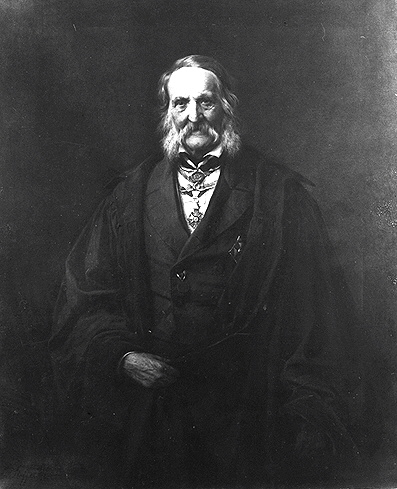
\includegraphics{bessel/figures/f_neumann}
  \caption{Franz Ernst (not John von) Neumann (1798 – 1895)}
\end{marginfigure}

From the theory of differential equations, it can be derived that Bessel's equation has two linearly independent solutions. One of them is the Bessel function of the first kind $J_\nu(x)$. It can be shown that a second independent solution is given by the Bessel function of the second kind defined by

\begin{equation}
\fbox{$\displaystyle
Y_\nu(x) = \frac{\cos(\nu \pi)J_\nu(x) - J_{-\nu}(x)}{\sin(\nu \pi)}
$}
\end{equation} 

This function is also called the \emph{Neumann} function, and is sometimes symbolised by $N_\nu(x)$.

Fig.~\ref{fig-bessel-Y} plots the Neumann functions of the lowest three orders. Note the logarithmic type singularity at $x=0$.

\begin{exer}
% difficulty: hard
The Neumann functions are supposed to be linearly independent from the Bessel functions. However, it seems like they are defined as linear combination of Bessel functions, as $\cos(\nu \pi)$ and $\sin(\nu \pi)$ are just numbers. What is going on? Focus your efforts on the case where $\nu$ is an integer.
\end{exer}

\begin{figure}
\centering
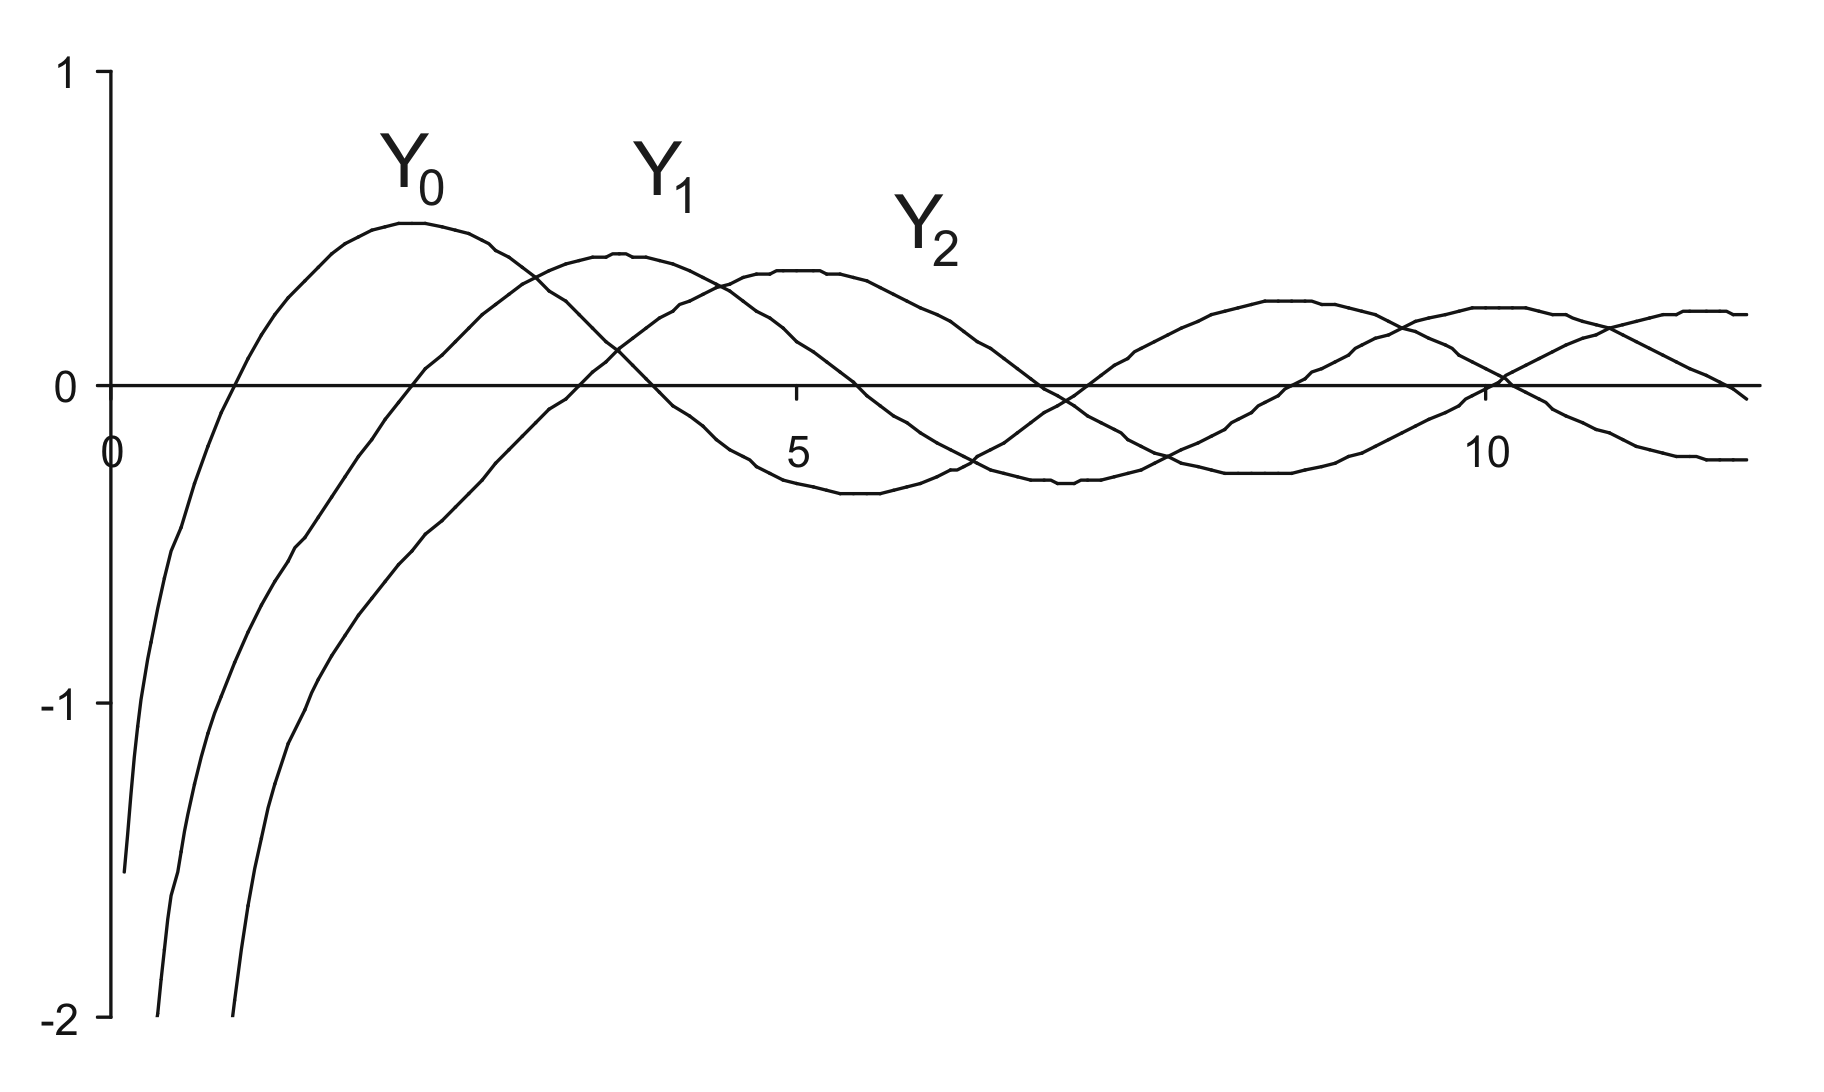
\includegraphics{bessel/figures/y}
\caption{The Neumann functions $Y_0(x)$, $Y_1(x)$ and $Y_2(x)$.}
\label{fig-bessel-Y}
\end{figure}

So the general solution of Bessel's equation can be written as

\begin{equation}
f(x) = A J_{\nu}(x) + B Y_{\nu}(x)
\end{equation} 

Obviously, any other linearly independent combination of $J_{\nu}(x)$ and $Y_{\nu}(x)$ can also be used to express the solution, e.g.

\begin{equation}
f(x) = C H_{\nu}^{(1)}(x) + D H_{\nu}^{(2)}(x)
\end{equation} 

\begin{marginfigure}[-1cm]
  % credits: Wikipedia
  % url: https://en.wikipedia.org/wiki/Hermann_Hankel
  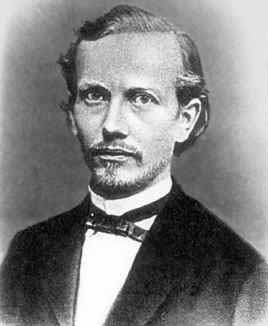
\includegraphics{bessel/figures/h_hankel}
  \caption{Hermann Hankel (1839–1873)}
\end{marginfigure}

Here, $H_{\nu}^{(1)}(x)$ and $H_{\nu}^{(2)}(x)$ are the \emph{Hankel} functions of the first and second kind respectively, defined by

\begin{subequations}
\begin{equation}
\fbox{$\displaystyle H_{\nu}^{(1)}(x) = J_{\nu}(x) + j Y_{\nu}(x)$}
\end{equation} 
\begin{equation}
\fbox{$\displaystyle H_{\nu}^{(2)}(x) = J_{\nu}(x) - j Y_{\nu}(x)$}
\end{equation} 
\label{eq-hankel}
\end{subequations} 

Of course, if we are solving Eq.~\ref{eq-helmholtz-cyl} instead of Eq.~\ref{eq-bessel}, the arguments of the functions above are $k_t r$ instead of $x$.

\pagebreak

\sectionugent{Cylindrical vs Cartesian wave solutions}

It is instructive to compare the Neumann and the Hankel functions to the solutions of the Helmholtz equation in a 1D Cartesian coordinate system:

\begin{equation}
f''(x) + k^2 f(x) = 0 \label{eq-helmholtz-1D}
\end{equation} 

The solutions of Eq.~\ref{eq-helmholtz-1D} are

\begin{equation}
f(x) = A \cos(kx) + B \sin(kx)
\end{equation} 

The sine and cosine solutions are oscillating solutions which can be interpreted physically as standing waves. Note the correspondence to $J_n(x)$ and $Y_n(x)$, which are also oscillating functions. Therefore, \textbf{Bessel and Neumann functions can be thought of as standing waves in a cylindrical coordinate system}. An important difference with respect to the geometric functions is of course that $Y_n(x)$ diverges at the origin.

\begin{exer}
% difficulty: trivial
% ugent
  It can be shown that for large arguments, the following asymptotic forms hold:
\begin{align}
J_\nu(x) \approx & \, \sqrt{\frac{2}{\pi x}} \cos \left( x - \left(\nu + \frac{1}{2}\right)\frac{\pi}{2} \right) \nonumber \\
Y_\nu(x) \approx & \, \sqrt{\frac{2}{\pi x}} \sin \left( x - \left(\nu + \frac{1}{2}\right) \frac{\pi}{2} \right)   
\end{align}

Purely based on the physics and the geometry of the problem, explain why it is plausible that sines and cosines appear here. If a source in the middle of a very large circular resonator excites a cylindrical standing wave, what will the wavefronts look like far from the source?

\end{exer}

Another way of writing the solutions of Eq.~\ref{eq-helmholtz-1D} is

\begin{equation}
f(x) = C e^{jkx} + D e^{-jkx}
\end{equation} 

because $e^{\pm j \theta} = \cos \theta \pm j \sin \theta$ (compare this to Eq.~\ref{eq-hankel}).

\pagebreak

\begin{exer}
% difficulty: trivial
% ugent
Does $e^{-jkx}$ correspond to an outgoing wave travelling towards $x=+\infty$, or to an incoming wave travelling towards $x=-\infty$?

How does the conclusion change if instead of  $e^{j \omega t}$ as time dependence in the definition of phasors, you chose $e^{-j \omega t}$?
\end{exer}


\begin{exer}
% difficulty: normal
% ugent
Show that for large arguments, the following asymptotic forms hold:
\begin{align}
H_{\nu}^{(1)} \approx & \, \sqrt{\frac{2}{\pi x}} e^{j \left( x - \left(\nu + \frac{1}{2}\right)\frac{\pi}{2} \right)} \nonumber \\
  H_{\nu}^{(2)} \approx & \, \sqrt{\frac{2}{\pi x}} e^{-j \left( x - \left(\nu + \frac{1}{2}\right)\frac{\pi}{2} \right)}
\end{align}

Based on physical and energy arguments, explain why the factor $1/\sqrt{x}$ is plausible. Remember that these functions will make up the electric and magnetic field components of solutions to the wave equation in cylindrical coordinates.
                          
\end{exer}

So, based on these observations, the \textbf{Hankel functions are the equivalent of travelling plane waves in a cylindrical coordinate system}.   $H_{\nu}^{(2)}(x)$ corresponds to an outgoing plane wave, while $H_{\nu}^{(1)}(x)$ \is an incoming plane wave (at least for our choice of time dependence).

Whether to use Bessel/Neumann functions or rather Hankel functions of the first and second kind to represent the solution of Bessel's differential equation, is usually determined by physical and/or practical considerations, as we will illustrate next for the case of finding eigenmodes in an optical fibre.


\pagebreak


\sectionugent{Application: the eigenmodes of an optical fibre}


\begin{marginfigure}
\centering
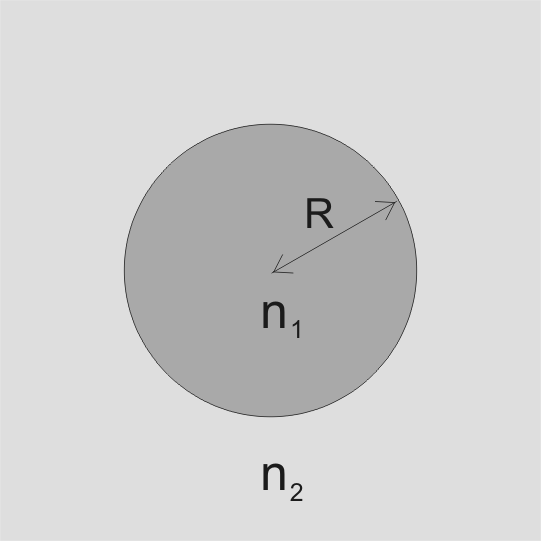
\includegraphics{bessel/figures/fibre}
\caption{Cross-section of an optical fibre.}
\label{fig-fibre}
\end{marginfigure}

Consider the optical fibre from Fig.~\ref{fig-fibre}: a central core with radius $R$ made of a material with refractive index $n_1$, surrounded by a cladding with refractive index $n_2 < n_1$. The cladding is taken to be infinitely thick. 

Fields in the optical fibre have to satisfy the Helmholtz equation. Just like in Section~\ref{sec-bessel-eq}, we propose solutions of the form 

\begin{equation}
\psi(r,\theta,z) = R(r)e^{-j k_\theta \theta }e^{-j k_z z} \\
\end{equation}

\begin{cue}
What is the physical interpretation of $k_z$? Also based on the physics of the problem, what can you say about $k_\theta $? Can it take any value?  
\end{cue}

These kinds of solutions are the eigenmodes of this particular waveguide, because of the form of their $z$--dependence\footnote{These eigenmodes propagate along $z$. Contrast this with the treatment of bent waveguides in the previous chapter, where the $z$--dimension didn't come in play because of the 2D nature of the problem and where the propagation was essentially along $\theta$.}.  Also, physics dictates that the fields must be periodic in the $\theta$--direction with period $2 \pi$. This means that the 'angular propagation constant' $k_\theta$ has to be an integer, which we will call $l = 0, \pm 1, \pm 2, \ldots$.

As we've seen before, $R$ has to satisfy this equation:

\begin{equation}
r^2\frac{d^2 R(r)}{d r^2} + r \frac{d R(r)}{d r} + \left[{r^2 \left(k_0^2 n^2(r) - k_z^2\right) - l^2}\right]R(r) = 0 \label{eq-fibre-0}
\end{equation} 

We define $k_{t,i}^2=k_0^2 n_i^2 - k_z^2$, where $i=1$ for the core and $i=2$ for the cladding.

\begin{exer}
% difficulty: trivial
% ugent
What is the physical meaning behind $k_t$? Draw a diagram. Contrast the diagram with Fig.~\ref{fig-fibre}.
\end{exer}

We already know that in each of the regions $i$, the solutions of Eq.~\ref{eq-fibre-0} are Bessel, Neumann or Hankel functions of order $l$ with argument $k_{t,i} r$.

\begin{cue}
For both the core and the cladding, what is the optimal way to represent the most general solution of the wave equation? In other words, which two linearly independent solutions in the family of Bessel, Neumann and Hankel functions should you choose, so that you can already put one contribution to zero because of the physics of the problem?
\end{cue}

For the core, we write the general solution as

\begin{equation}
R(r) = A J_l\left(k_{t,1}r\right) + B Y_l\left(k_{t,1}r\right), \hspace{0.5 cm} r<R \label{eq-fibre-1}
\end{equation} 

But since the Neumann functions diverge at $r=0$, and we don't observe any infinite fields in the centre of an optical fibre, it immediately follows that $B=0$.

For the cladding, it is more advantageous to write the general solution in terms of Hankel functions:

\begin{equation}
R(r) = C H_l^{(1)}\left(k_{t,2}r\right) + D H_l^{(2)}\left(k_{t,2}r\right), \hspace{0.5 cm} r>R \label{eq-fibre-2}
\end{equation} 

For physical reasons, there can only be outgoing waves towards infinity, not incoming waves from infinity. Indeed, there are neither sources nor reflectors at infinity in our situation. So, this means that $C=0$.

\begin{exer}
% difficulty: trivial
% ugent
For guided modes, where $k_0 n_2 < k_z < k_0 n_1$, use the asymptotic expansion of the Hankel functions to show that the fields are exponentially decaying in the cladding.
\end{exer}

If we have weakly guided fibres where $n_1 \approx n_2$, it turns out that the continuity conditions of the electric and the magnetic fields can be approximated by imposing the continuity of $R$ and $d R / d r$.

\begin{cue}
Impose these conditions, and derive an expression from which we can calculate the propagation constants $k_z$. 
\end{cue}

Imposing the continuity of $R$ and $d R / dr$ leads to

\begin{equation}
A J_l\left(k_{t,1}R\right) = D H_l^{(2)}\left(k_{t,2}R\right)
\end{equation} 

\begin{equation}
A k_{t,1} J'_l\left(k_{t,1}R\right) = D k_{t,2} H_l'^{(2)}\left(k_{t,2}R\right)
\end{equation} 

This only has non--trivial solutions if

\begin{equation}
\frac{J_l\left(k_{t,1}R\right)}{k_{t,1} J'_l\left(k_{t,1}R\right)} = \frac{H_l^{(2)}\left(k_{t,2}R\right)}{k_{t,2} H_l'^{(2)}\left(k_{t,2}R\right)} \label{eq-disp-fibre}
\end{equation}

Since $k_{t,1}$ and $k_{t,2}$ are functions of $k_z$, Eq.~\ref{eq-disp-fibre} has effectively only a single unknown $k_z$ for a given geometry. We can therefore use that equation to calculate the propagation constants of the eigenmodes of the fibre.

Once the propagation constants are found, the field profiles can be calculated from Eq.~\ref{eq-fibre-1} and \ref{eq-fibre-2}.


\begin{exer}
% difficulty: normal
Solve the Helmholtz equation in free space in cylindrical coordinates. Look at the evolution of the intensity of the solution as a function of $z$. What do you notice? These modes are called \emph{Bessel beams}.
\end{exer}



\section*{Review questions}

\begin{itemize}
\item What are Bessel functions?  
\item How can a generating function be used to define Bessel functions?
\item What techniques can you use to solve integrals of the product of Bessel functions with a polynomial?
\item What is a Fourier-Bessel series expansion and how can it be used?
\item Under what scalar product are Bessel functions orthogonal?
\item What are Neumann functions?
\item What are Hankel functions?
\item What is the correspondence between solutions of the Cartesian wave equation and the cylindrical one?   
\end{itemize}

%%% Local Variables:
%%% mode: latex
%%% TeX-master: "../main"
%%% End:
